\documentclass{beamer}
 
\usepackage{fontawesome}
\usepackage[utf8]{inputenc}
\usepackage{minted}

\usetheme{Madrid}
\setbeamertemplate{itemize subitem}[square]

\title{A very informal introduction to Python}
\author{Federico Galatolo}
\date{}
\titlegraphic{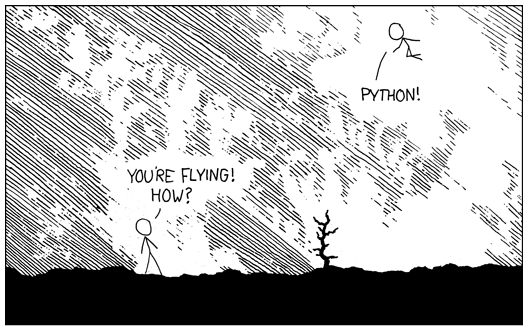
\includegraphics[width=.5\textwidth,height=.4\textheight]{imgs/python.png}}

\newcommand{\pyfuncname}[2]{\texttt{\textunderscore\textunderscore#1\textunderscore\textunderscore#2}}

\begin{document}

\frame{\titlepage}

\begin{frame}
    \frametitle{Python}
    \begin{figure}
        
\includegraphics[scale=0.3]{imgs/logo.png}
    \end{figure}
    \begin{itemize}
        \item Object Oriented
        \item Multiple Inheritance
        \item Dynamically Typed
        \item Large built-in libraries
        \item Free (as in freedom) and Open Source
    \end{itemize}
\end{frame}

\begin{frame}
    \frametitle{Why Python?}
    \begin{figure}
        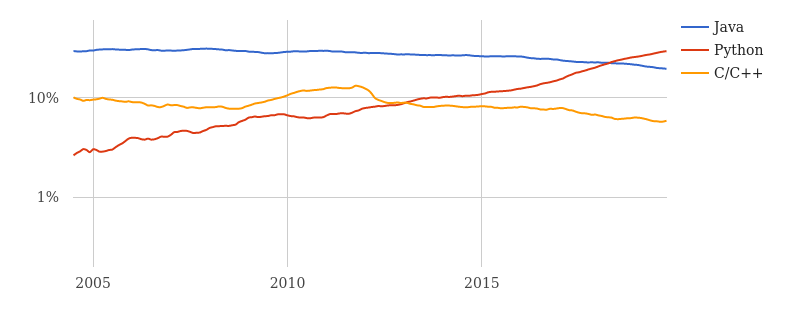
\includegraphics[scale=0.3]{imgs/stats.png}
        \caption{Languages popularity over time}
    \end{figure}
    \begin{itemize}
        \item High Level
        \item Portable (Actually write once run everywhere)
        \item Extendible in C/C++
        \item Easy to learn and maintain
    \end{itemize}
\end{frame}


\begin{frame}
    \frametitle{PyPI: The Python Package Index}
    \begin{figure}
        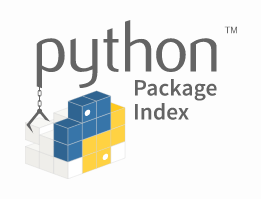
\includegraphics[scale=0.3]{imgs/pipy.png}
    \end{figure}
    \begin{itemize}
        \item Over 200.000 packages
        \item Over 400.000 developers
        \item Portable packages
        \item Managed by a Non-Profit Organization
        \item Open Source
    \end{itemize}
\end{frame}

\begin{frame}
    \frametitle{Virtual Environments (1)}
    \begin{figure}
        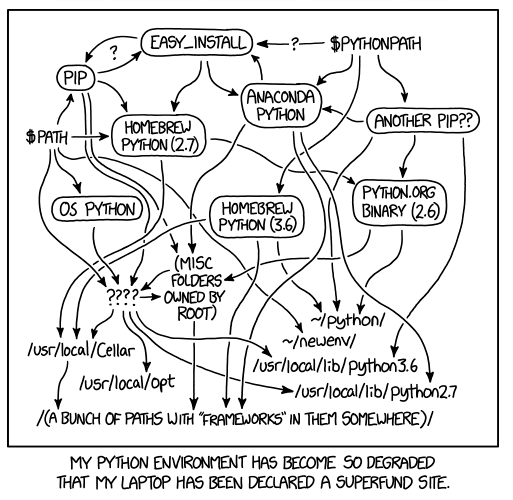
\includegraphics[scale=0.25]{imgs/xkcd.png}
    \end{figure}
    \begin{itemize}
        \item Method for having project-wide dependencies
        \item Without it everything become very messy in very little time
        \item All the dependencies are stored in a folder
        \item The dependencies folder can be easily snapshotted and retrieved
    \end{itemize}
\end{frame}

\begin{frame}
    \frametitle{Virtual Environments (2)}
    \begin{itemize}
        \item Create a Virtual Environment with python \texttt{X.Y} in folder \texttt{env}
        \begin{itemize}
            \item \texttt{virtualenv --python=pythonX.Y env}
        \end{itemize}
        \item Activate the Virtual Environment
        \begin{itemize}
            \item \texttt{source ./env/bin/activate}
            \item \texttt{. ./env/bin/activate}
        \end{itemize}
        \item Deactivate the Virtual Environment
        \begin{itemize}
            \item \texttt{deactivate}
        \end{itemize}        
    \end{itemize}
\end{frame}

\begin{frame}
    \frametitle{Managing Packages}
    \begin{itemize}
        \item Install \texttt{package}
        \begin{itemize}
            \item \texttt{pip install \texttt{package}}
        \end{itemize}
        \item Uninstall \texttt{package}
        \begin{itemize}
            \item \texttt{pip uninstall \texttt{package}}
        \end{itemize}
        \item Snapshot installed packages in \texttt{requirements.txt}
        \begin{itemize}
            \item \texttt{pip freeze > requirements.txt}
        \end{itemize}        
        \item Install all packages snapshotted in \texttt{requirements.txt}
        \begin{itemize}
            \item \texttt{pip install -r requirements.txt}
        \end{itemize}
    \end{itemize}
\end{frame}

\begin{frame}[fragile]{Built-in types}
    Python is \textbf{dynamically typed}.\\
    Variables types are determined at \textbf{runtime}.\\
    Variables can freely change type during the execution.\\
    In python there are a lot of built-in types, the most notables are:
    \begin{itemize}
        \item Boolean (\texttt{bool})
        \item Strings (\texttt{str})
        \item Numbers (\texttt{int}, \texttt{float})
        \item Sequences (\texttt{list}, \texttt{tuple})
        \item Mapping (\texttt{dict})
    \end{itemize}
    There is still hope to have a coherent codebase with \textbf{dynamic type checking} (last slides)
\end{frame}

\begin{frame}[fragile]{Variables assignement}
    As you might expect variables are assigned like this:
    \begin{minted}{python}
        pi = 3 # problems?
        name = "Federico"
    \end{minted}
    You can assign multiple variables at once with \textbf{iterable unpacking}.
    \begin{minted}{python}
        pi, name = 3, "Federico"
        first, second, third = SomeSequence
    \end{minted}
    In python \textbf{everything} is stored and passed as \textbf{reference} with the only exception of Numbers.
    \begin{minted}{python}
        a = [1, 2, 3]
        b = a
        b[0] = 5 # now a = [5, 2, 3]
    \end{minted}
\end{frame}

\begin{frame}[fragile]{Block syntax: hate it or love it}
    In python you \textbf{don't} surround code blocks with curly brackets\\
    You just use \textbf{indentation}\\
    \begin{itemize}
        \item C like syntax
        \begin{minted}{c}
        for(int i = 0; i < n; i++){
            int k = i % 3
            if(k == 0){
                // stuff...
            }
        }
        \end{minted}
        \item Python syntax
        \begin{minted}{python}
        for i in range(0, n):
            k = i % 3
            if k == 0:
                # stuff...
        \end{minted}
    \end{itemize}
\end{frame}


\begin{frame}[fragile]
    \frametitle{Conditional instructions(1)}
    Simple conditional instruction with the \textbf{if} keyword.
    \begin{minted}{python}
    if someConditions:
        someActions()
        someOtherActions()
    \end{minted}
    Python uses \textbf{and} and \textbf{or} as logical operators instead of \textbf{\&\&} and \textbf{$\vert\vert$}
    \begin{minted}{python}
        if (C1 and C2) or C3:
            someActions()
            someOtherActions()
    \end{minted}
\end{frame}

\begin{frame}[fragile]
    \frametitle{Conditional instructions(2)}
    The \textbf{else} statement works as you might expect:
    \begin{minted}{python}
        if Condition:
            someActions()
        else:
            someOtherActions()
    \end{minted}

    There is no \textbf{switch case} statement in python. You can use \textbf{if} and \textbf{elif}
    \begin{minted}{python}
        if C1:
            A1()
        elif C2:
            A2()
        elif C3:
            A3()
        else:
            A()
    \end{minted}
\end{frame}

\begin{frame}[fragile]
    \frametitle{Conditional instructions(3): Inline}
    Inline conditional instructions works as you might expect.\\
    The python syntax is:
    \begin{minted}{python}
        value if Condition else otherValue
    \end{minted} 
    For example:
    \begin{minted}{python}
        pi = 3 if isEngineer else 3.1415
    \end{minted} 
    
\end{frame}


\begin{frame}[fragile]
    \frametitle{While loops}
    The while loops works as you might expect:
    \begin{minted}{python}
        while Conditions:
            Stuff()
            otherStuff()
    \end{minted}
    There \textbf{is no} do-while construct in python.
\end{frame} 

\begin{frame}[fragile]
    \frametitle{For loops(1)}
    In python the for loop \textbf{is} a \textbf{for each}.
    \begin{minted}{python}
        for element in elements:
            doStuff(element)
    \end{minted}
    \texttt{elements} must be and \texttt{Iterable}.\\
    \hfill \\
    You can use \texttt{tuple unpacking} in for loops: 
    \begin{minted}{python}
        for x, y in SequenceOfTuples:
            doStuff(x, y)
    \end{minted}
\end{frame}

\begin{frame}[fragile]
    \frametitle{For loops(2): useful built-ins}
    With \textbf{zip()} you can combine \textbf{one-by-one} the elements of two or more \texttt{iterables} 
    \begin{minted}{python}
        L1 = [1, 2, 3]
        L2 = [4, 5, 6]
        for x, y in zip(L1, L2): 
            print(x, y)
    \end{minted}
    \hfill \\
    \textbf{enumerate()} will return a list of \texttt{(index, element)} tuples: 
    \begin{minted}{python}
        names = ["Federico", "Mario", "Giovanni"]
        for i, name in enumerate(names):
            print(i, name)
    \end{minted}
\end{frame}

\begin{frame}[fragile]
    \frametitle{For loops(3): list comprehension}
    The python equivalent for inline for loop it is called  list comprehension.\\
    It is \textbf{not} a for loop but a way for building a list, the syntax is
    \begin{minted}{python}
        [someOperation(element) for element in elements]
    \end{minted}
    For example:
    \begin{minted}{python}
        squares = [i**2 for i in range(0, N)]
    \end{minted}
\end{frame}

\begin{frame}[fragile]
    \frametitle{Functions(1)}
    You can define a new function using the \texttt{def} keyword
    \begin{minted}{python}
        def getCircleArea(r):
            return pi*r**2
    \end{minted}
    Default arguments values are indicated with \texttt{=}
    \begin{minted}{python}
        def getCircleArea(r, isEngineer=True):
            pi = 3 if isEngineer else 3.1415
            return pi*r**2
    \end{minted}
\end{frame}

\begin{frame}[fragile]
    \frametitle{Functions(2): Variable positional arguments}
    You can define a \textbf{variable} number of arguments with the \texttt{*} symbol
    \begin{minted}{python}
        def sumOfSquares(*args):
            squares = [arg**2 for arg in args]
            return sum(squares)
    \end{minted}
    Calling the function like this:
    \begin{minted}{python}
        result = sumOfSquares(1, 2, 3)
    \end{minted}
\end{frame}

\begin{frame}[fragile]
    \frametitle{Functions(3): Sequence dereference}
    Likewise you can pass sequences as positional arguments in this way:  
    \begin{minted}{python}
        def norm2D(x, y):
            return math.sqrt(x**2 + y**2)
        
        vec = [2, 3]
        norm = norm2D(*vec)
    \end{minted}
\end{frame}

\begin{frame}[fragile]
    \frametitle{Functions(4): Keyword arguments}
    Besides positional arguments python has \textbf{keyword} arguments\\
    You can specify that a function uses keyword arguments with the \texttt{**} symbol.\\
    You \textbf{must} use that symbol as last argument  
    \begin{minted}{python}
def greet(language = "en", **kwargs):
    if language == "it":
        print("Ciao "+kwargs["name"]+" "+kwargs["surname"])
    else:
        print("Hello "+kwargs["name"]+" "+kwargs["surname"])

greet("it", surname="Galatolo", name="Federico")
greet(name="Mario", surname="Cimino")
    \end{minted}
\end{frame}

\begin{frame}[fragile]
    \frametitle{Functions(5): Dictionary dereference}
    As you might have guessed you can pass a \texttt{dict} of keyword arguments using the symbol \texttt{**}
    \begin{minted}{python}
def greet(language = "en", **kwargs):
    if language == "it":
        print("Ciao "+kwargs["name"]+" "+kwargs["surname"])
    else:
        print("Hello "+kwargs["name"]+" "+kwargs["surname"])

person = dict(name="Federico", surname="Galatolo")
greet("it", **person)
greet(**person)
    \end{minted}
\end{frame}

\begin{frame}[fragile]
    \frametitle{Bonus: Iterators and Generators}
    \texttt{Iterables} are objects that implement the \pyfuncname{iter}{()} to get an \texttt{Iterator}\\
    \texttt{Iterators} are object that implement the \pyfuncname{next}{()} to get the next element\\
    \texttt{Generators} are a kind of \texttt{Iterators} in which the elements are evaluated \textbf{on-the-fly}\\
    \hfill \\
    You can define an inline generator with the \texttt{list comprehension} syntax but using the parenthesis instead of the square brackets.
    \begin{minted}{python}
        squares = (i**2 for i in range(0, N))
    \end{minted}
\end{frame}



\begin{frame}[fragile]
    \frametitle{Functions(6): yield}
    Using the \texttt{yield} statement stead of the return the function returns a \texttt{Generator}.\\
    The elements outputted by the generator are the elements yielded by the function.\\
    The yield \textbf{does not} stop the execution flow of the function it just yield a value and go on.\\
    \begin{minted}{python}
    def counter(i, end):
        while i < end:
            yield i
            i += 1
    \end{minted}
\end{frame}

\begin{frame}[fragile]
    \frametitle{Functions(7): Inline}
    You can create inline functions using the \texttt{lambda} keyword.\\
    The syntax is 
    \begin{minted}{python}
        lambda comma, separated, arguments : expression
    \end{minted}
    For example
    \begin{minted}{python}
        norm2D = lambda x, y: math.sqrt(x**2 + y**2)
    \end{minted}
\end{frame}


\begin{frame}[fragile]
    \frametitle{Classes(1)}
    In python classes are defined with the \texttt{class} keyword.\\
    Class methods are defined with the \texttt{def} keyword.\\
    Every method \texttt{must have} one argument.\\
    When a method is called from an instance the first argument is a reference to the caller instance.\\
    Conventionally the name of the first argument is \texttt{self}.\\
    \begin{minted}{python}
    class Person:
        def getName(self):
            return "Federico"
        def greet(self):
            return "Hi! I am "+self.getName()
    \end{minted}
\end{frame}

\begin{frame}[fragile]
    \frametitle{Classes(2): Instance attributes}
    In python you can create, modify and retrieve instance attributes using the dot (\texttt{.}) selector on the instance reference.\\
    You can create and assign an instance attribute everywhere in a class method.
    \begin{minted}{python}
    class Person:
        def setName(self, name):
            self.name = name
        def greet(self):
            return "Hi! I am "+self.name
    \end{minted}
\end{frame}

\begin{frame}[fragile]
    \frametitle{Classes(3): Class attributes aka static attributes}
    You can create class attributes specifying them after the class declaration. 
    You can modify and retrieve class attributes using the dot (\texttt{.}) selector on the class reference
    \begin{minted}{python}
    class Person:
        greeting = "Hi!"
        def setName(self, name):
            self.name = name
        def greet(self):
            return Person.greeting+" I am "+self.name
    \end{minted}
\end{frame}

\begin{frame}[fragile]
    \frametitle{Classes(4): Class methods aka static methods}
    You can specify class method as a normal class method without the first argument (it make sense if you think about it)
    \begin{minted}{python}
    class Person:
        greeting = "Hi!"
        def getGreeting():
            return Person.greeting
    
    g = Person.getGreeting()
    \end{minted}
\end{frame}


\begin{frame}[fragile]
    \frametitle{Classes Bonus: It is all about notation}
    ``Nothing is true, everything is permitted''\\
    Python does not know about static/non-static methods, it is all about notation
    \begin{minted}{python}
    class Person:
        greeting = "Hi!"
        def setName(self, name):
            self.name = name
        def greet(self):
            return Person.greeting+" I am "+self.name
    
    p = Person()
    p.greet() # ok
    Person.greet(p) # still ok
    \end{minted}
\end{frame}



\begin{frame}[fragile]
    \frametitle{Classes(5): Visibility}
    In python there \textbf{is no} such thing as a \textbf{private} method or attribute.\\
    Everything is \textbf{public}\\
    \hfill \\
    The naming convention for ``private'' methods and attributes is to precede their name with the \texttt{\textunderscore} symbol.
    \begin{minted}{python}
    class Person:
        def setName(self, name):
            self._name = name
        def greet(self):
            return "Hi! I am "+self._name
    \end{minted}
\end{frame}


\begin{frame}[fragile]
    \frametitle{Classes(6): Constructor}
    In python the construct function is named \pyfuncname{init}{} and it is called at object instantiation.\\
    You can specify \textbf{one or more arguments}.\\
    As for all the python methods the first one is the object instance reference.\\
    \begin{minted}{python}
    class Person:
        def __init__(self, name):
            self._name = name
        def greet(self):
            return "Hi! I am "+self._name
    p = Person("Federico")
    \end{minted}
\end{frame}

\begin{frame}[fragile]
    \frametitle{Classes(7): Inheritance}
    You can extend a base class with another specifying the base class between the parenthesis at class definition
    \begin{minted}{python}
    class Person:
        def __init__(self, name):
            self._name = name
        def greet(self):
            return "Hi! I am "+self._name
    
    class Student(Person):
        def greet(self):
            return "Leave me alone, I have to study"
    \end{minted}
\end{frame}


\begin{frame}[fragile]
    \frametitle{Classes(8): Data model}
    The are a lot of built-in functions provided by the base class of all the classes \texttt{object}.\\
    Each of which provide a specific behavior, a few are:\\
    \begin{itemize}
        \item \pyfuncname{len}{(self)}
        \begin{itemize}
            \item Returns the ``length'' of the object (called by \texttt{len()})
        \end{itemize}
        \item \pyfuncname{str}{(self)}
        \begin{itemize}
            \item Returns the object as a \texttt{string} (called by \texttt{str()})
        \end{itemize}
        \item \pyfuncname{lt}{(self, other)}, \pyfuncname{lt}{(self, other)}, \pyfuncname{eq}{(self, other)}, ...
        \begin{itemize}
            \item Called when the object is used in a comparison 
        \end{itemize}
        \item \pyfuncname{getitem}{(self, key)}, \pyfuncname{setitem}{(self, key, value)}, 
        \begin{itemize}
            \item Called in square brackets access
        \end{itemize}
    \end{itemize}
\end{frame}

\begin{frame}[fragile]
    \frametitle{Classes(9): Inheritance done well}
    When extending a base class you might need to call its construct or its methods.\\
    In order to get the base class class reference you need to use the \texttt{super()} function
    \begin{minted}{python}
    class Student(Person):
        def __init__(self, name):
            super(Student).__init__(self)

        def greet(self):
            return "Leave me alone, I have to study"
    \end{minted}
    Keep in mind that \mintinline{python}{super(Class)} returns the base class reference.\\
    And that \mintinline{python}{super(Class, self)} returns the base class instance.\\
    e.g. \mintinline{python}{super(Class).__init__(self)} is the same as \mintinline{python}{super(Class, self).__init__()}
\end{frame}


\begin{frame}[fragile]
    \frametitle{Classes(10): Inheritance tips and tricks}
    Keyword arguments are usually preferred over positional ones.\\
    Since \texttt{kwargs} is a \texttt{dict} each construct should pop out its own keys a forward the others.\\
    \begin{minted}{python}
    class Person:
        def __init__(self, **kwargs):
            self.name = kwargs.pop("name")
    
    class Student(Person):
        def __init__(self, **kwargs):
            self.grade = kwargs.pop("grade")
            super(Student, self).__init__(**kwargs)
    \end{minted}
\end{frame}

\begin{frame}[fragile]
    \frametitle{Bonus: Arguments subtleties}
    Default arguments can be passed as keyword arguments
    \begin{minted}{python}
    def greet(name="Federico", surname="Galatolo"):
        return "Hi "+name+" "+surname

    greet(surname="Cimino", name="Mario")
    \end{minted}
\end{frame}

\begin{frame}[fragile]
    \frametitle{Bonus: Dynamic type checking}
    In python 3 PEP 484 introduced dynamic type checking syntax to python
    \begin{minted}{python}
    def greet(name: str, isFriend: bool = False) -> str:
        return "Hi "+name if isFriend else "Hello "+name
    \end{minted}
    It is \textbf{just a syntax}.\\
    If you want to run dynamic type checking at run time you need to run a \textbf{type checker} (for example \texttt{mypi}).\\
    \hfill \\
    PEP stays for Python Enhancement Proposal and they are the RFCs of python
\end{frame}


\begin{frame}
    \frametitle{That's all folks!}
    \begin{center}
        You can find the slides PDF as well as their \LaTeX \;source code on GitHub. \\
        \hfill \\
        https://github.com/galatolofederico/python-very-informal-introduction
    \end{center}
    \hfill \\
    \hfill \\
    \begin{columns}
        \begin{column}{.5\textwidth}
            \begin{itemize}
                \item [\faEnvelope] federico.galatolo@ing.unipi.it
                \item [\faPaperPlane] @galatolo
            \end{itemize}
        \end{column}
        \begin{column}{.5\textwidth}
            \begin{itemize}
                \item [\faGlobe] galatolo.me
                \item [\faGithub] @galatolofederico
            \end{itemize}
        \end{column}
    \end{columns}
\end{frame}


\end{document}